\documentclass[a4paper,11pt]{book}
\usepackage[utf8]{inputenc}
\usepackage{fullpage}
\usepackage[backend=bibtex8]{biblatex}
\usepackage[autostyle]{csquotes}
\usepackage[dutch]{babel}
\usepackage{vub}
\usepackage{sansmath}
\usepackage{hyperref}
\usepackage{float}
\usepackage{multirow}

\restylefloat{table} % om om tabellen niet te laten herpositioneren
\raggedbottom
\let\cleardoublepage\clearpage

% VUB huisstijl voor font en kleur
\color{pantone418}
\renewcommand{\familydefault}{\sfdefault}
\sansmath

\bibliography{build/refs}

\begin{document}

\frontmatter
%VUB-voorblad configureren
\author{Nicolas Carraggi, Youri Coppens, Christophe Gaethofs, Pieter Meiresone, Sam Van den Vonder, Fernando Suarez, Tim Witters}
\title{Vergadering XX/XX/XX}
\subtitle{Software Engineering} 
\faculty{Faculteit Ingenieurswetenschappen \& Wetenschappen}
\date{Academiejaar 2013-2014}


\makeassignment
\chapter{Versiegeschiedenis}

\begin{table}[htbp]
	\centering
	\caption{Versiegeschiedenis}
	\begin{tabular} {|c|c|c|c|}
	    \hline
		\textbf{Versie} & \textbf{Datum} 	& \textbf{Auteur(s)} & \textbf{Commentaar} \\
		\hline
		1.0	& 30/11/2013	& Sam Van den Vonder & Initi\"{e}le versie \\ \hline
		1.1 & 10/12/2012	& Sam Van den Vonder & Aanpassingen kwaliteitsinspectie \\ \hline
	\end{tabular}
\end{table}

\tableofcontents
\listoffigures
\listoftables

\mainmatter
\chapter{Introductie}

\section{Doel}
Dit document beschrijft de softwarearchitectuur en het design van de CalZone webapplicatie.
\section{Scope}

\section{Acroniemen}

\begin{table}[H]
	\centering
	\caption{Acroniemen}
	\label{tab:Acroniemen}
	\begin{tabular}{l | l}
	
	API	& Application Programming Interface\\

	DB	& Database\\

	GUI	& Graphical User Interface\\

	JSP & Java Server Page\\

	MVC & Model View Controller\\ 

	SDD	& Software Design Description\\

	SDK	& Software Development Kit\\

	SRS	& Software Requirements Specification\\
	
	XML & Extensible Markup Language\\
	
	\end{tabular}
\end{table}


\section{Overzicht}
Dit document volgt de IEEE Std 1016-2006\texttrademark \space standaard voor het opstellen van Software Design Descriptions. 
Dit document is be\"{i}nvloed door de requirements beschreven in de Software Requirements Specification van dit project.\\ In de huidige fase van dit document wordt het design van het systeem in de eerste iteratie beschreven. 
\chapter{Systeemarchitectuur}
\label{chap:architectuur}

\section{Model}
\label{sec:model}
CalZone is een webapplicatie. Gebruikers van het systeem bezoeken de applicatie via hun webbrowser. 
Deze browser kan de browser op hun computer zijn of de webbrowser op hun smartphone.
Doorheen de ontwikkeling van het project wordt de focus vooral gericht op Android toestellen en browsers op deze toestellen wat betreft het mobiele aspect van de applicatie.
\\
CalZone heeft als architectuur gekozen voor het MVC-patroon.\cite{mvc}

\begin{figure}[H]
	\centering
	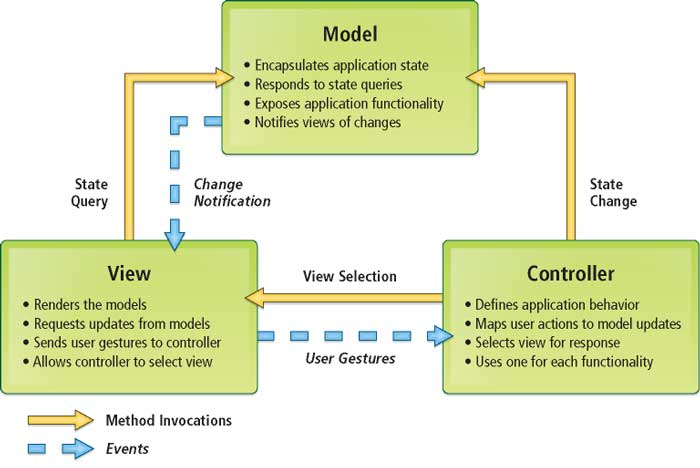
\includegraphics[scale=0.5]{img/mvc}
	\label{fig:mvc}
	\caption{Een voorstelling van de werking van een systeem gebruikmakende van een MVC architectuur}
\end{figure}

\section{Gebruikte technologie}
\label{sec:technologie}
De programmeertaal die gebruikt wordt, is Java. 
In Java wordt gebruik gemaakt van het Spring MVC framework\cite{spring, spring-mvc} voor het ontwikkelen van CalZone. 
De IDE waarin geprogrammeerd wordt, is de meest recente versie van 'Eclipse Classic' met volgende uitbreidingen:

\begin{itemize}
	\item De gehele collectie 'Web, XML, Java EE and OSGi Enterprise Development'	
	\item Spring Tool Suite (uit de Eclipse Marketplace)
	\item De gehele collectie 'Maven Integration for Eclipse'
\end{itemize}
\noindent
Het uitvoeren van de applicatie wordt mogelijk gemaakt door middel van Apache Maven\cite{Maven} en Apache Tomcat\cite{Tomcat}.
De gebruikte databank voor de back-end is MySQL.
De connecties vanuit het logisch niveau van het systeem naar de databank verloopt via Hibernate\cite{hibernate} 
Voor de view wordt gebruik gemaakt van JSP's: een technologie om dynamisch webpagina's te genereren.

\chapter{Modules}

\nocite{*}
\printbibliography

\end{document}